% small.tex
\documentclass[12pt]{beamer}
\usetheme{amcg}
\beamertemplatenavigationsymbolsempty
\renewcommand{\thefootnote}{}
\providecommand{\e}[1]{\ensuremath{\times 10^{#1}}}
\usepackage{mathptmx}
\usepackage{helvet}
\usepackage{color}
\newcommand\TILDE{\char`\~}
\usepackage{listings}

% items enclosed in square brackets are optional; explanation below
\title[Fluidity]{Downloading and building Fluidity}
\subtitle[]{}
\institute{1 - Dept of Earth Science and Engineering, Imperial College London}
\author[Dave Robinson]{\large{Dave Robinson}\inst{1}}
\date{}


\begin{document}


%--- the titlepage frame -------------------------%
\begin{frame}
  \titlepage
\end{frame}

%-- Overview slide --- %
\section*{Outline}
\begin{frame}
  \frametitle{Outline}
  \tableofcontents
\end{frame}

\begin{frame}
        \frametitle{Today...}
...we will learn how to:
\begin{itemize}
    \item Build Fluidity
    \item Make a mesh
    \item Set up a Fluidity simulation
    \item Run a Fluidity simulation
    \item Look at the output
    \item Run Fluidity in parallel
\end{itemize}
\end{frame}


\section{Getting Fluidity}
\begin{frame}
        \frametitle{Where to get Fluidity}
\begin{itemize}
    \item {\bf Binary} (release only)
	  \\Prebuilt Debian package available through wajig, apt-get, etc.
    \item {\bf Source} (release, trunk or branch)
	  \\Download using bzr commands, accessing Launchpad.
    \item {\bf Archived} (release only)
	  \\Tarballed release source code (.tgz)
\end{itemize}
\end{frame}

\begin{frame}[fragile]
        \frametitle{Downloading the Release binary}
\lstset{language=bash}
{\centering{\color{red} *** please don't do this bit now ***}}
\begin{lstlisting}[language=bash,basicstyle=\ttfamily\small]
sudo apt-add-repository -y ppa:fluidity-core/ppa
sudo apt-get update
sudo apt-get -y install fluidity
\end{lstlisting}
The binary of Fluidity requires no compiling or building and will be updated automatically by apt-get.
\end{frame}

\begin{frame}[fragile]
        \frametitle{Downloading the Release source}
\lstset{language=bash}
{\centering{\color{red} *** please don't do this bit now ***}}
\\ Alternatively, the source code for the release can be accessed using bzr.
\begin{lstlisting}[language=bash,basicstyle=\ttfamily]
bzr co lp:fluidity/4.1 fluidity-release/
\end{lstlisting}    
This will require configuring and building, which we will cover later.
\end{frame}

\begin{frame}[fragile]
        \frametitle{Downloading the Trunk source}
\lstset{language=bash}
The source code for the trunk (or any branch) can also be accessed using bzr.
\begin{lstlisting}[language=bash,basicstyle=\ttfamily]
bzr co lp:fluidity/ fluidity/
\end{lstlisting}    
\end{frame}


\begin{frame}
        \frametitle{Launchpad}
\begin{center}
    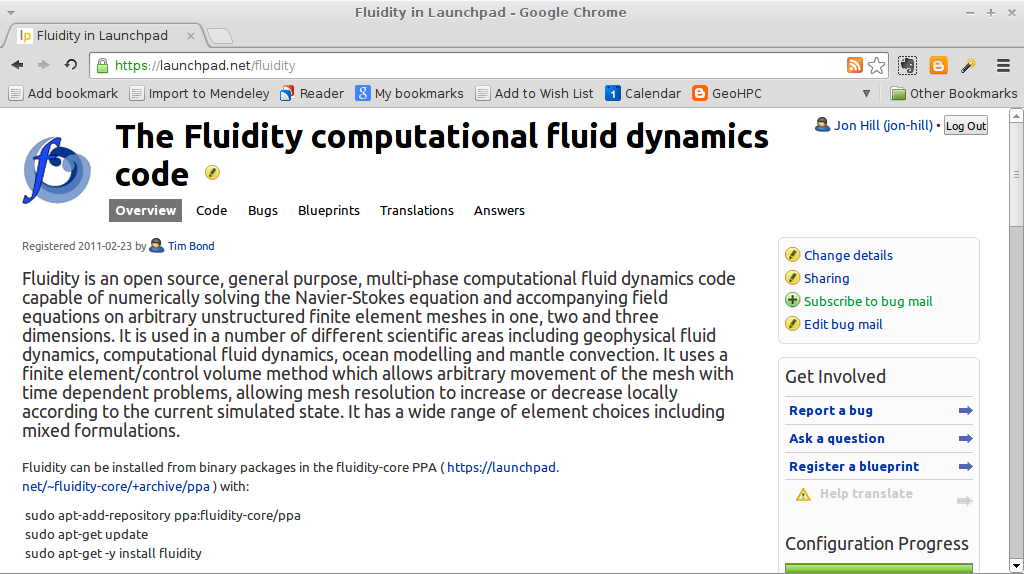
\includegraphics[width=0.9\textwidth]{images/launchpad-home.png}
\end{center}
http://launchpad.net/fluidity
\end{frame}
\begin{frame}
        \frametitle{Launchpad}
\begin{center}
    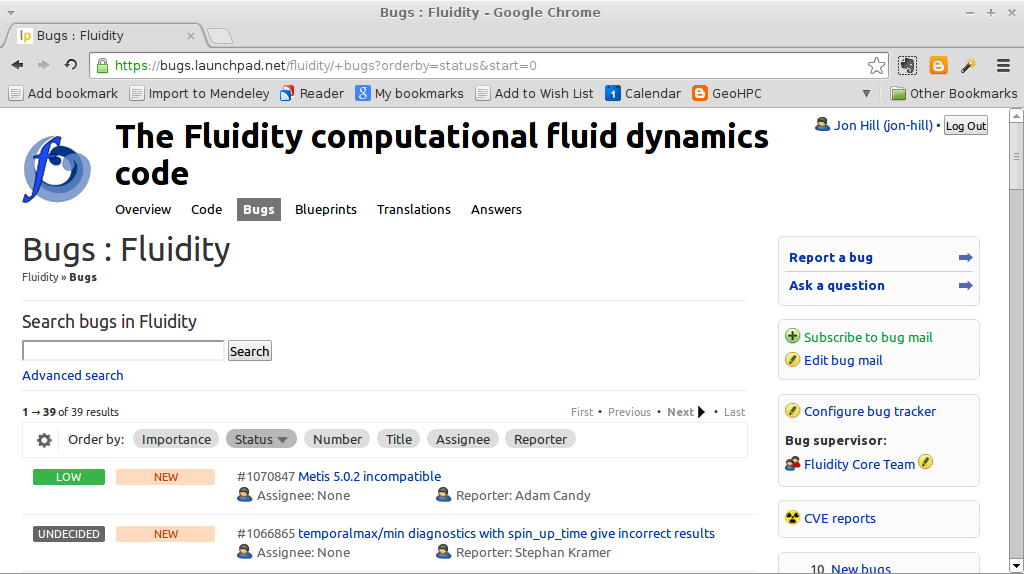
\includegraphics[width=0.9\textwidth]{images/launchpad-bugs.png}
\end{center}
http://launchpad.net/fluidity
\end{frame}
\begin{frame}
        \frametitle{Launchpad}
\begin{center}
    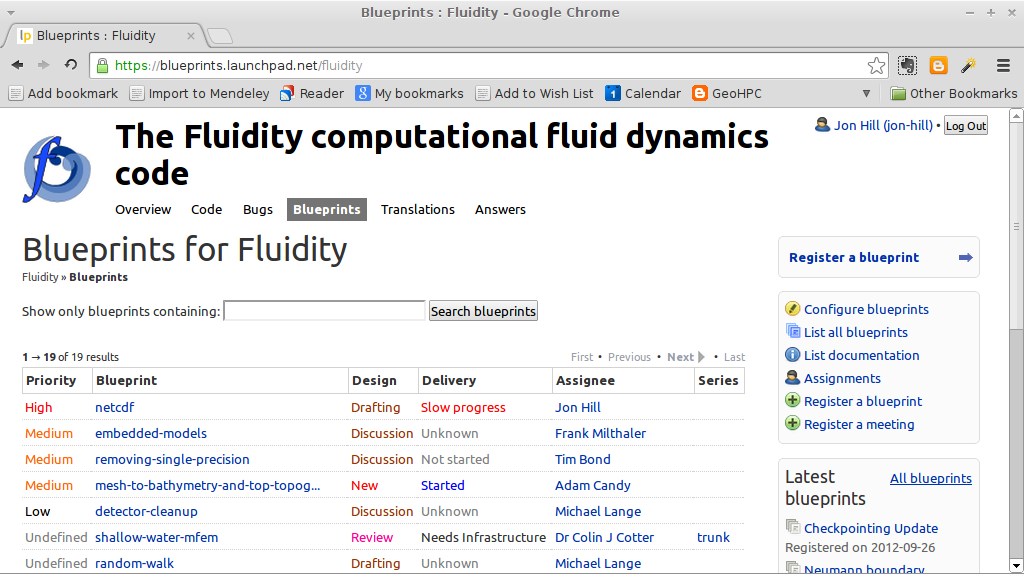
\includegraphics[width=0.9\textwidth]{images/launchpad-blueprint.png}
\end{center}
http://launchpad.net/fluidity
\end{frame}
\begin{frame}
        \frametitle{Launchpad}
\begin{center}
    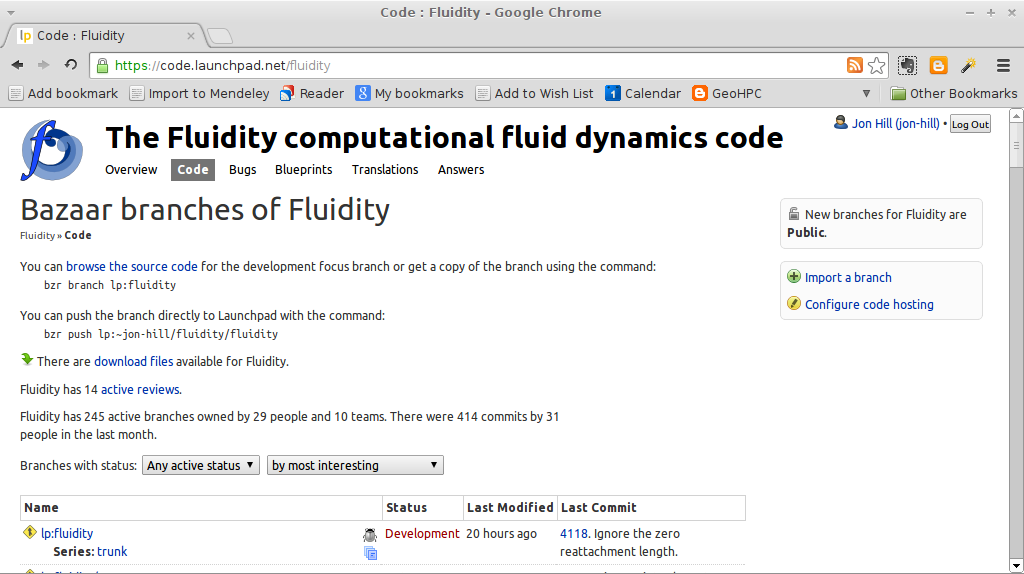
\includegraphics[width=0.9\textwidth]{images/launchpad-code.png}
\end{center}
http://launchpad.net/fluidity
\end{frame}
\begin{frame}
        \frametitle{Launchpad}
\begin{center}
    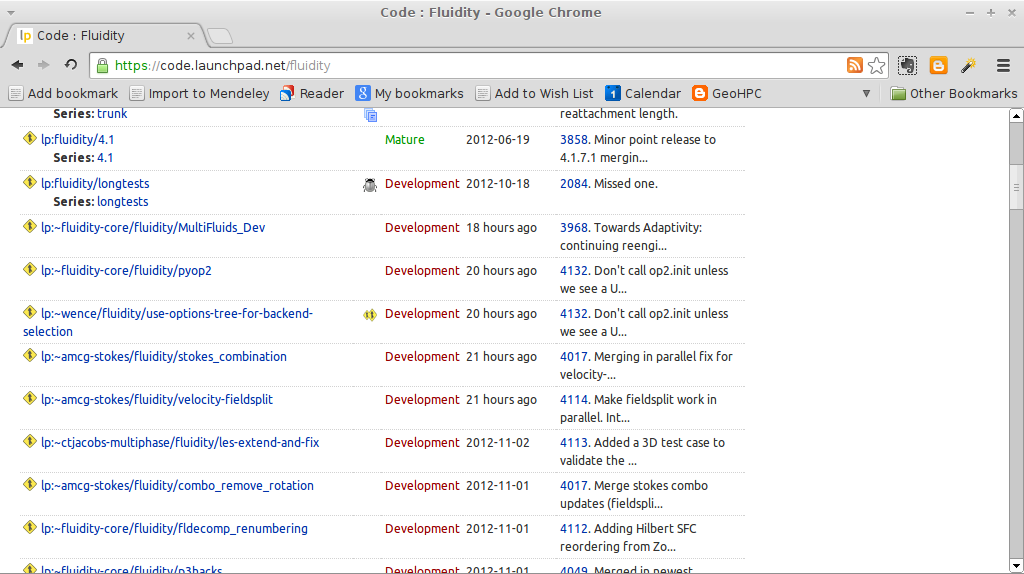
\includegraphics[width=0.9\textwidth]{images/launchpad-code2.png}
\end{center}
http://launchpad.net/fluidity
\end{frame}

\begin{frame}
\frametitle{Buildbot}
\begin{center}
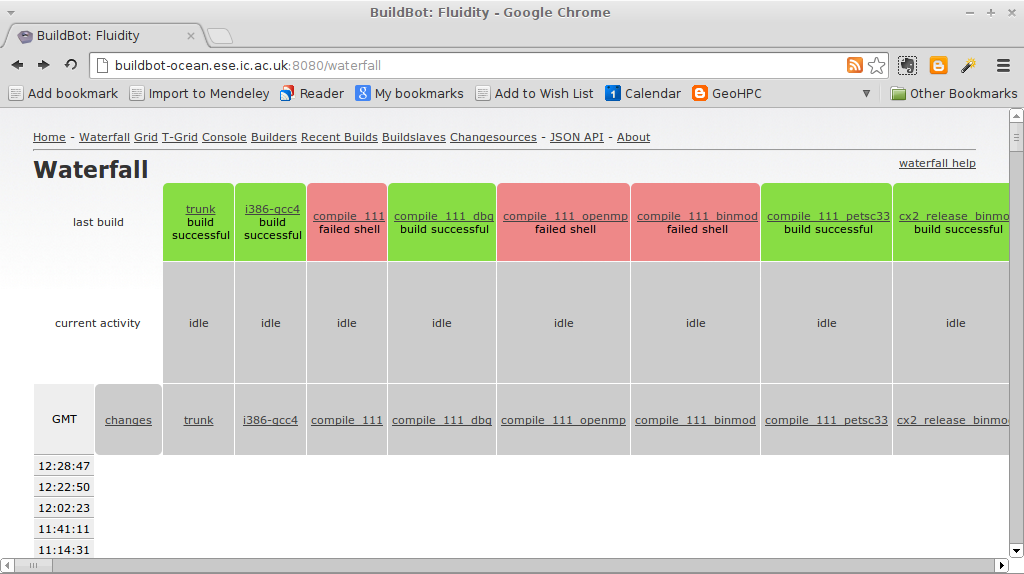
\includegraphics[width=0.9\textwidth]{images/buildbot.png}
\end{center}
http://buildbot-ocean.ese.ic.ac.uk:8080/waterfall
\end{frame}

\section{Configuring and building}
\begin{frame}[fragile]
        \frametitle{Configure}
Set up compile-time options, such as:
\begin{itemize}
    \item External non-LGPL libraries
    \item Non-standard libray locations
    \item Compiler flags
    \item Debugging
\end{itemize}
\lstset{language=bash}
\begin{lstlisting}[language=bash,basicstyle=\ttfamily]
module load petsc-gcc4
cd [fluidity directory]
./configure --enable-2d-adaptivity
\end{lstlisting}
\end{frame}

\begin{frame}[fragile]
        \frametitle{Building}
\lstset{language=bash}
\begin{lstlisting}[language=bash,basicstyle=\ttfamily]
make clean && make -j 4 && make fltools
\end{lstlisting}
\end{frame}

\begin{frame}[fragile]
    \frametitle{Python}
\lstset{language=bash}
Fluidity contains several Python packages that are required for it to run.  
The Fluidity python directory must be added to the existing environment variable PYTHONPATH.
\begin{lstlisting}[language=bash,basicstyle=\ttfamily\footnotesize]
export PYTHONPATH=$PYTHONPATH:/data/fluidity/python
\end{lstlisting}
This can be checked by using the echo command.
\begin{lstlisting}[language=bash,basicstyle=\ttfamily\footnotesize]
echo $PYTHONPATH
\end{lstlisting}
\end{frame}

\section{Installing}
\begin{frame}[fragile]
        \frametitle{Tests}
\lstset{language=bash}
If you wished to check that a particular build of Fluidity passes the group's library of verification tests then you can use one of these commands.

{\center{\color{red} *** please don't do this bit now ***}}
\begin{lstlisting}[language=bash,basicstyle=\ttfamily]
make unittest
make test
make mediumtest
\end{lstlisting}
\end{frame}

\begin{frame}[fragile]
        \frametitle{Installing}
\lstset{language=bash}
Installing Fluidity enables access for all other users of your computer.
\begin{lstlisting}[language=bash,basicstyle=\ttfamily]
make install
make install-diamond
make install-user-schemata
\end{lstlisting}
\end{frame}

\begin{frame}
    \frametitle{Running Fluidity}
From source:    
\\ \texttt{[fl. dir.]/bin/fluidity -v2 -l [filename].flml}
\\ [0.5cm]
From binary:    
\\ \texttt{fluidity -v2 -l [filename].flml}
\end{frame}

\begin{frame}[fragile]
        \frametitle{Updating}
\lstset{language=bash}
\begin{lstlisting}[language=bash,basicstyle=\ttfamily]
bzr up
    
M preprocessor/Populate_State.F90
\end{lstlisting}

\begin{lstlisting}[language=bash,basicstyle=\ttfamily]
bzr status
bzr status -SV
bzr diff filename
\end{lstlisting}
\end{frame}

\begin{frame}[fragile]
    \frametitle{edit \textasciitilde /.bashrc}
.bashrc is a file run everytime you open a new terminal.
\\ \vspace{10pt}
\texttt{cd}
\\ \texttt{gedit .bashrc \&}
\\ \vspace{10pt}
Go to the end of the file and add the following lines:
\\ \vspace{10pt}
\texttt{module load petsc-gcc4}
\\ \texttt{export PYTHONPATH=\$PYTHONPATH:/data/[your username]/fluidity/python}

\end{frame}

\end{document}

